\documentclass[uplatex, dvipdfmx]{jsarticle}
% \documentclass[uplatex,dvipdfmx, titlepage]{jsarticle}
% \usepackage[top=2.5cm, bottom=2.5cm]{geometry}
\usepackage{amsmath,amssymb,amsthm}
\usepackage{mathtools}
\usepackage{mathrsfs}
\usepackage{graphicx}
\usepackage{here}
\usepackage{enumerate}
\usepackage{algorithm}
\usepackage{algpseudocode}
\usepackage{colortbl}
\usepackage{color}
\usepackage{listings}
\usepackage{tikz}
\usepackage{hyperref}
\usepackage{circuitikz}
\usepackage{fancyvrb}

\usetikzlibrary{arrows}
\usetikzlibrary{shapes.geometric}
\usetikzlibrary{positioning}
\usetikzlibrary{intersections, calc, arrows}

\newtheoremstyle{case}{}{}{}{}{}{:}{ }{}
\theoremstyle{case}
\newtheorem{case}{Case}

\DeclareMathOperator*{\argmin}{arg\,min}
\DeclareMathOperator*{\argmax}{arg\,max}
\DeclareMathOperator*{\rank}{rank}
\DeclareMathOperator{\Ima}{Im}

\newcommand{\transposed}[1]{#1^\mathsf{T}}

\newtheorem{lemma}{Lemma}
\newtheorem{theorem}{Theorem}
\newtheorem{proposition}{Proposition}
\newtheorem{definition}{Definition}

\title{
  計数工学プログラミング演習 レポート課題
  % \begin{Large}
  %   「数値解析」
  % \end{Large}
  % \begin{large}
  %     Aセメスター 月4 \教員: 松尾 宇泰 先生\
  % \end{large}
  % \vspace{15pt}
  % \begin{Large}
  %     期末レポート課題\
  % \end{Large}
  % \vspace{20pt}
  % \begin{Huge}
  %   多項式係数補間アルゴリズムの比較
  %   % Precision comparison of\
  %   % polynomial coefficients interpolation
  % \end{Huge}
  % \vspace{100pt}
}

\author{
  % \begin{Large}
    03-210634 木下裕太
  % \end{Large}
}

\begin{document}
  \maketitle

  \section{目的}
  疎行列の2乗を計算し、実行時間を測定する。
  実装方法の違いによって、速度にどのような差が生じるかを調べる。

  \section{方法}
  2つの実装 Dense および Sparse に対して比較を行う。
  計算量についてはスカラーの四則演算が単位時間で行えると仮定。

  \subsection{Dense implementation}
  2次元配列として行列を管理する。
  行列積は定義に基づいたシンプルな実装であり、疑似コードは以下のようになる。
  $n$を行列のサイズとして、時間計算量は$\Theta(n^3)$、空間計算量は$\Theta(n^2)$である。

  \begin{algorithm}[h]
    \centering
    \caption{Dense version}
    \begin{algorithmic}[1]
      \Require
      \Statex $A$ : $n\times n$行列
      \Ensure
      \Statex 返り値は$A^2$。
      \Function{SquareDense}{$A$}
      \State $B\gets O_n$
      \For{$i = 1, \cdots ,n$}
      \For{$k = 1, \cdots ,n$}
      \For{$j = 1, \cdots ,n$}
      \State $B_{i,j} \gets B_{i,j} + A_{i,k}A_{k,j}$
      \EndFor
      \EndFor
      \EndFor
      \State \Return $B$
      \EndFunction
    \end{algorithmic}
  \end{algorithm}

  \subsection{Sparse implementation}
  全ての行と列について、含まれる非ゼロ成分を可変長リストで管理する。
  行列積の実装は先とほぼ同様だが、非ゼロ成分のみにアクセスする工夫をしている。
  疑似コードは以下の通りである。
  $m$を非ゼロ成分の個数とすると、時間計算量$O(nm)$で動作する。
  \footnote{各非ゼロ成分は高々2回参照される。}

  \begin{algorithm}[h]
    \centering
    \caption{Sparse version}
    \begin{algorithmic}[1]
      \Function{SquareSparse}{$A$}
      \State $B\gets O_n$
      \For{$k = 1, \cdots ,n$}
      \For{$A_{i,k}\neq 0$}
      \For{$A_{k,j}\neq 0$}
      \State $B_{i,j} \gets B_{i,j} + A_{i,k}A_{k,j}$
      \EndFor
      \EndFor
      \EndFor
      \State \Return $B$
      \EndFunction
    \end{algorithmic}
  \end{algorithm}

  \subsection{実行環境}
  以下の実行環境で測定を行う。
  \begin{table}[h]
    \centering
    \begin{tabular}{l|c}
      CPU & Intel(R) Core(TM) i5-8250U, 1.60GHz \\
      RAM & 8 GB\\
      OS & Windows 10 (64 bit)\\
      Language & C (GCC 10.3.0)\\
    \end{tabular}
  \end{table}

  \subsection{サンプルケース}
  \href{https://math.nist.gov/MatrixMarket/matrices.html}{Matrix Market}のデータを入力として用いる。
  今回は疎行列のみを対象として測定を行う。
  各入力について10回繰り返し実行させ、所要時間の平均をその入力に対する実行速度とする。

  \newpage
  \section{実験結果}
  縦軸、横軸ともに対数スケールである。
  なお2つのコードの出力が全てのケースで一致することを確認した。

  \begin{figure}[h]
    \centering
    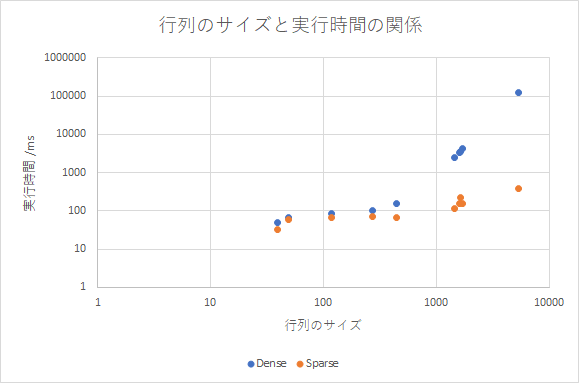
\includegraphics[scale=1.2]{fig.png}
  \end{figure}

  \section{考察}
  予想される通り、$m\in o(n^2)$である入力に対してSparseの方がオーダーレベルで高速だった。
  今回の実装は一般に2つの疎行列の積を計算する場合にもそのまま同様に適用できるが、
  一方で2つの行列が同じであるという特殊な設定を上手く活かすことができなかった。
\end{document}
